\documentclass[12pt,twoside,letterpaper]{article}
\usepackage{graphicx}
\usepackage{amsmath}
\usepackage{float}

\begin{document}
\title{Cutting a Spur Gear on the Van Norman 16 Mill}
\author{Andrew Young}
\date{6/1/2018}


\maketitle

\begin{abstract}
This document describes the process of replicating a spur gear using a Van Norman 16 milling machine. The instructions are intended for technical students or hobbyists interested in making a replacement gear via horizontal milling.
\end{abstract}

\clearpage

\tableofcontents

\section{Introduction}

This manual will walk you through creating a replacement gear using a Van Norman 16 milling machine, with a horizontal dividing head by the same manufacturer. The methods described herein apply specifically to straight-toothed spur gearing using the inch standard. 

\subsection{ Time Needed}

The speed of the process depends on the number of teeth to be cut and the skill of the operator. Generally, you should plan on taking your time, maybe 5 minutes per tooth starting out, plus setup and cleanup time. For a 16-tooth gear, that might be about 2 hours, provided all materials are at hand.


\subsection{Overview}

This manual will take you through the steps of measuring a gear and replicating it on a Van Norman milling machine. 


Please read and understand the operator manual for the mill - all relevant information for gear cutting will be included here, but you should consult the manufacturer's manual for matters such as routine lubrication and maintenance of the mill.


In addition, you will need to make or procure a cylindrical blank for cutting the gear teeth into. Determining the dimensions of the blank will be part of subsection 1, but the turning of the blank on the lathe is outside of the scope of this manual.


The steps for gear replication are, broadly:

\begin{enumerate}
\item Measure the gear that is desired to be replicated
\item Machine Setup
\item Gear Cutting
\item Verifying Measurements
\item Cleanup
\end{enumerate}


\subsection{Disclaimer}

The author of this manual disclaims liability for any damages caused by the use, or misuse of the information in the manual. This process involves operating a machine tool under power, and as such, there is a grave risk of personal injury if undertaken by someone who is not adequately informed, or worse, is not adequately attentive to the risks inherent in the task. 

If you feel you are unsure of how to conduct any step in a safe, controlled manner, please go take a class from a qualified instructor, and do not rely on this manual as a sole instructive device. 


\subsection{ Needed Items and Resources}

The following tools and materials will be needed to make a replacement gear. Many of the exact sizes needed for tools will depend on the gear being cut - see subsection 1 for the procedure determining how to choose cutters, arbors, and measuring tools appropriately.

Tools Needed: 

\begin{enumerate}
\item Van Norman 16 Milling Machine
\item Van Norman 10" horizontal index head
\item Index Plate
\item Cutter arbor fitting a VN 'C' taper
\item Mandrel for gear blank
\item Lathe Dog for Mandrel
\item Gear Cutter
\item S.A.E Wrenches
\item Gear measuring wires
\item Micrometer of appropriate size or calipers (micrometer preferred)
\item Acid brush or coolant system
\end{enumerate}


\subsubsection{Materials}

\begin{enumerate}
\item Gear example to copy
\item Gear blank of appropriate size (calculate size using procedure in subsection 1)
\item Cutting oil or coolant of choice
\end{enumerate}

\subsection{ Dangers, Warnings, Cautions, and Notes}

\begin{enumerate}
\item Do NOT attempt to cut gearing without coolant or lubricant, with the exception of cast iron gearing. Doing so will reduce tool life significantly. 
\item Machine tools are dangerous. Observe standard shop safety procedures including wearing eye protection and hearing protection, if necessary. Keep hands away from moving parts. 
\item Read all instructions thoroughly before attempting to follow procedure.
\item Ensure procedure is followed carefully and double-check setups before running under power. Failure to do so may result in a machine crash and, under certain circumstances, severe injury or death.
\end{enumerate}




\subsection{An Orientation to The Mill}


You should be familiarized with all basic controls of the milling machine, having read the manufacturer's instruction manual. The images from the manual pointing out the major features are reproduced here for convenience.


\begin{figure}[H]
	\centering
		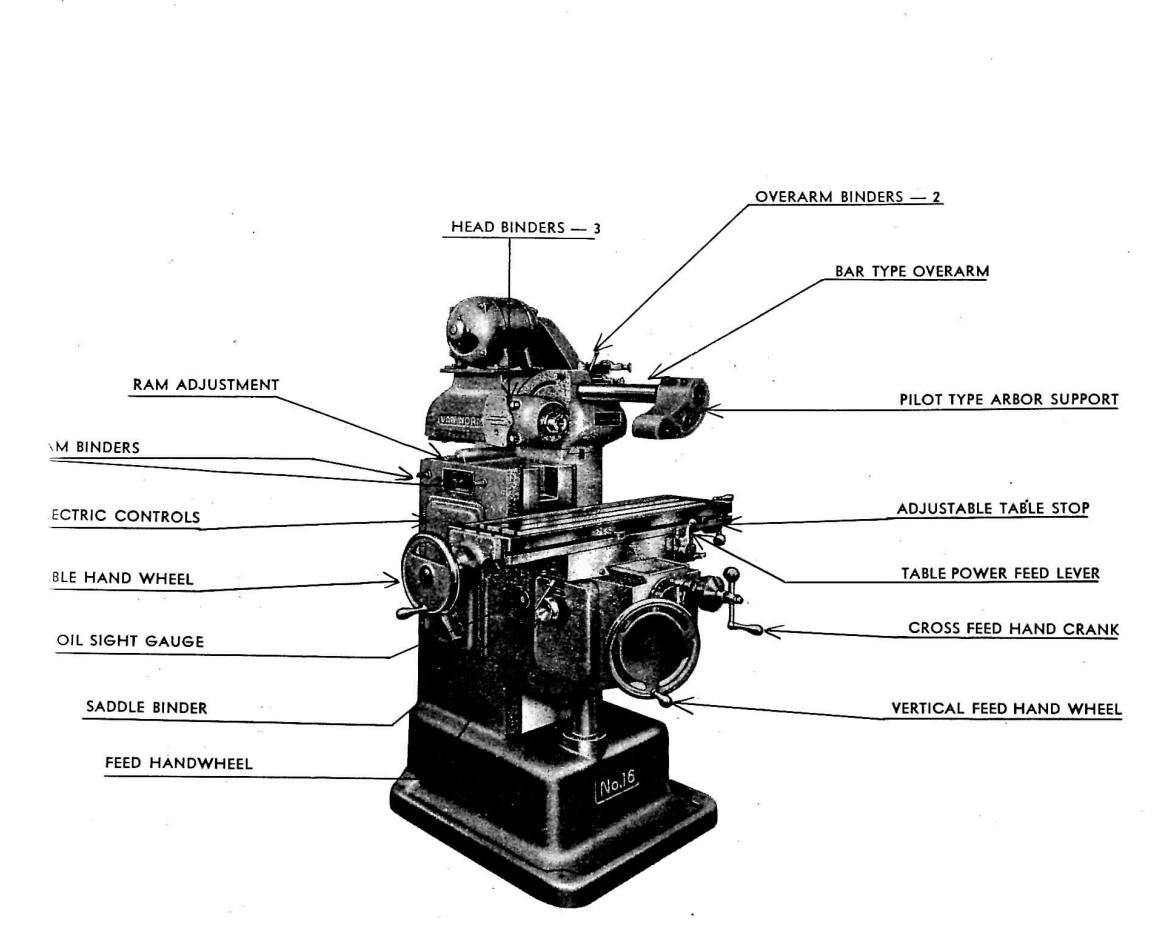
\includegraphics[width=5in]{diagram1}
\caption{Mill image 1. Adapted from ``Installation, Operation, and Maintenance Instructions and Parts List for No. 16 Van Norman Ram Type Milling Machine Plain and Universal Models" [Pamphlet]. (1952). Springfield, MA: Van Norman Company. }
\end{figure}

\begin{figure}[H]
	\centering
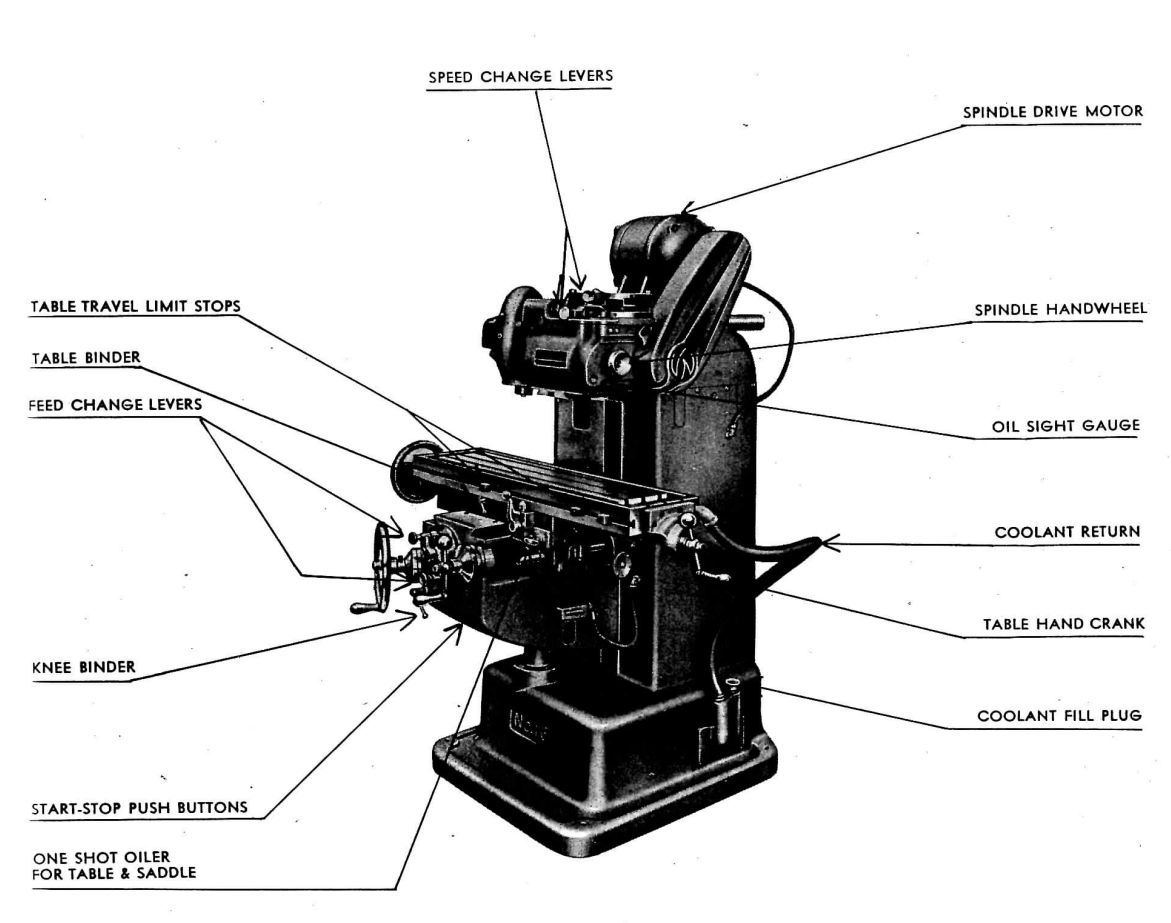
\includegraphics[width=5in]{diagram2}
\caption{Mill image 2. Adapted from ``Installation, Operation, and Maintenance Instructions and Parts List for No. 16 Van Norman Ram Type Milling Machine Plain and Universal Models" [Pamphlet]. (1952). Springfield, MA: Van Norman Company. }
\end{figure}


\section{Measuring the Gear}

In order to measure and discuss gearing sensibly, a few terms are needed. Gearing is perhaps surprisingly complicated if you haven't run into the terminology used before.

\begin{figure}[H]
	\centering

\includegraphics[width=5in]{imgpending}
\caption{Photo of this operation to be taken later this weekend.}
\end{figure}


\subsection{Gears: an extension of the wheel.}


It is helpful to think of a gear as an extension of a wheel - in fact, watchmakers still call gears 'wheels.' When two gears fit together (called ``meshing,'') there is an imaginary circle that can be drawn over each gear where it touches the teeth of the other gear or gears that it meshes with. This imaginary circle is called the ``pitch circle.''

\begin{figure}[H]
\centering
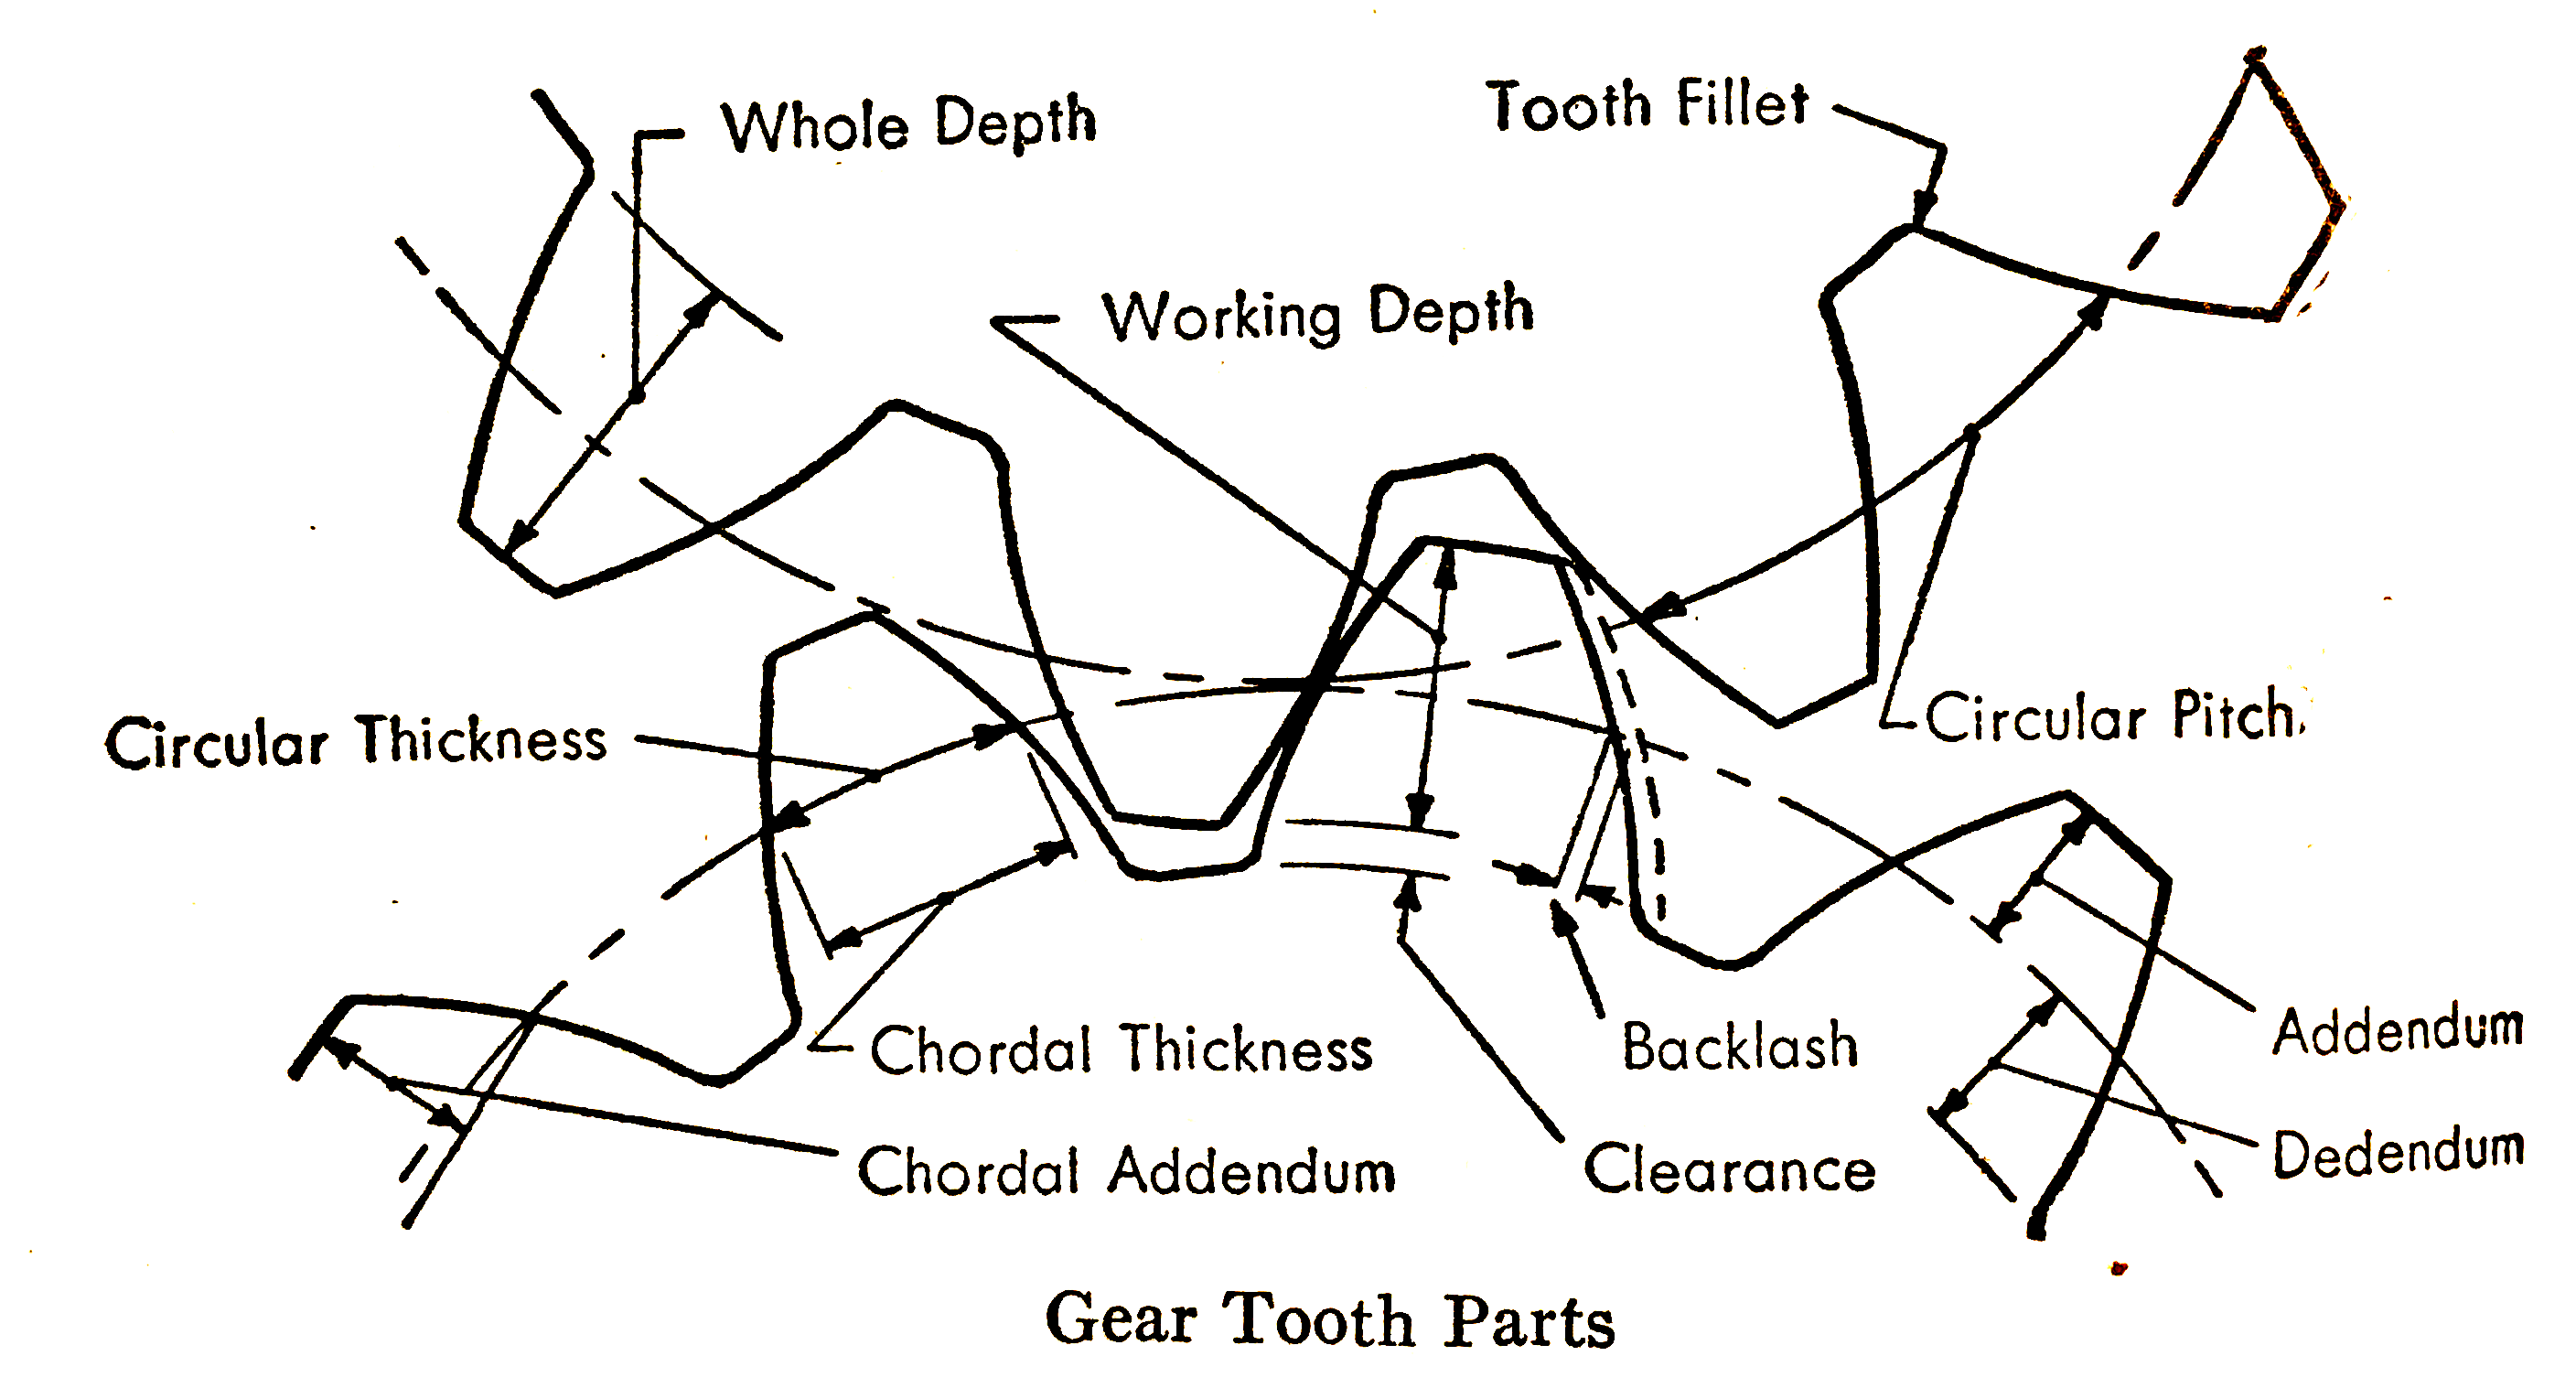
\includegraphics[width=5in]{gearparts1}
	\caption{Gear Tooth Parts. Adapted from Horton, H. L. (Ed.). (1954). Machinery's Handbook (15th ed.). New York, NY: The Industrial Press. }
\end{figure}


\subsection{Critical Measurements}
\begin{enumerate}
\item Number of Teeth. Count the teeth around the rim of the gear and write this down.
\item Pitch Circle. Find the approximate distance between the outside of a tooth on one side of the gear, and the inside diameter of the gear teeth on the other. This is about the size of the pitch circle - an approximate measure is OK here.
\item Thickness of Gear
\item Bore diameter of Gear. Record the diameter of the bore.
\item Diametral Pitch. Find the diametral pitch by taking the number of teeth on the gear and dividing it by the pitch diameter. The pitch diameter will probably have to be approximated - find a circle about halfway between the inner and outer diameter of the gear. In our example case, we will be cutting a 16dp, or 16 diametral pitch gear, which is a relatively common size.


\subsection{Making the Blank}
\begin{figure}[H]
\centering

\includegraphics[width=5in]{imgpending}
	\caption{Gear blank for example project.}
\end{figure}
		Making the gear blank is beyond the scope of this manual, but should fall well within the expertise of anyone familiar with lathe work. The keyway is an important part, which may be broached, filed, or shaped, depending on the materials at hand. Tolerances required for gear blanks are fairly tight - for a run-of-the-mill part, one or two thousandths maximum should be held on the main bore of the blank. If a particularly good class of work is desired, Machinery's handbook has the relevant tolerances in tabular form (Horton, 1954).

\end{enumerate}

\subsection{Tooling Choices}
\subsubsection{Choosing the Cutter}
The cutter is to be chosen based on the diametral pitch and the number of teeth to be cut. Once you have a set of cutters for your given diametral pitch, you will notice they are numbered:

\begin{figure}[H]
\centering
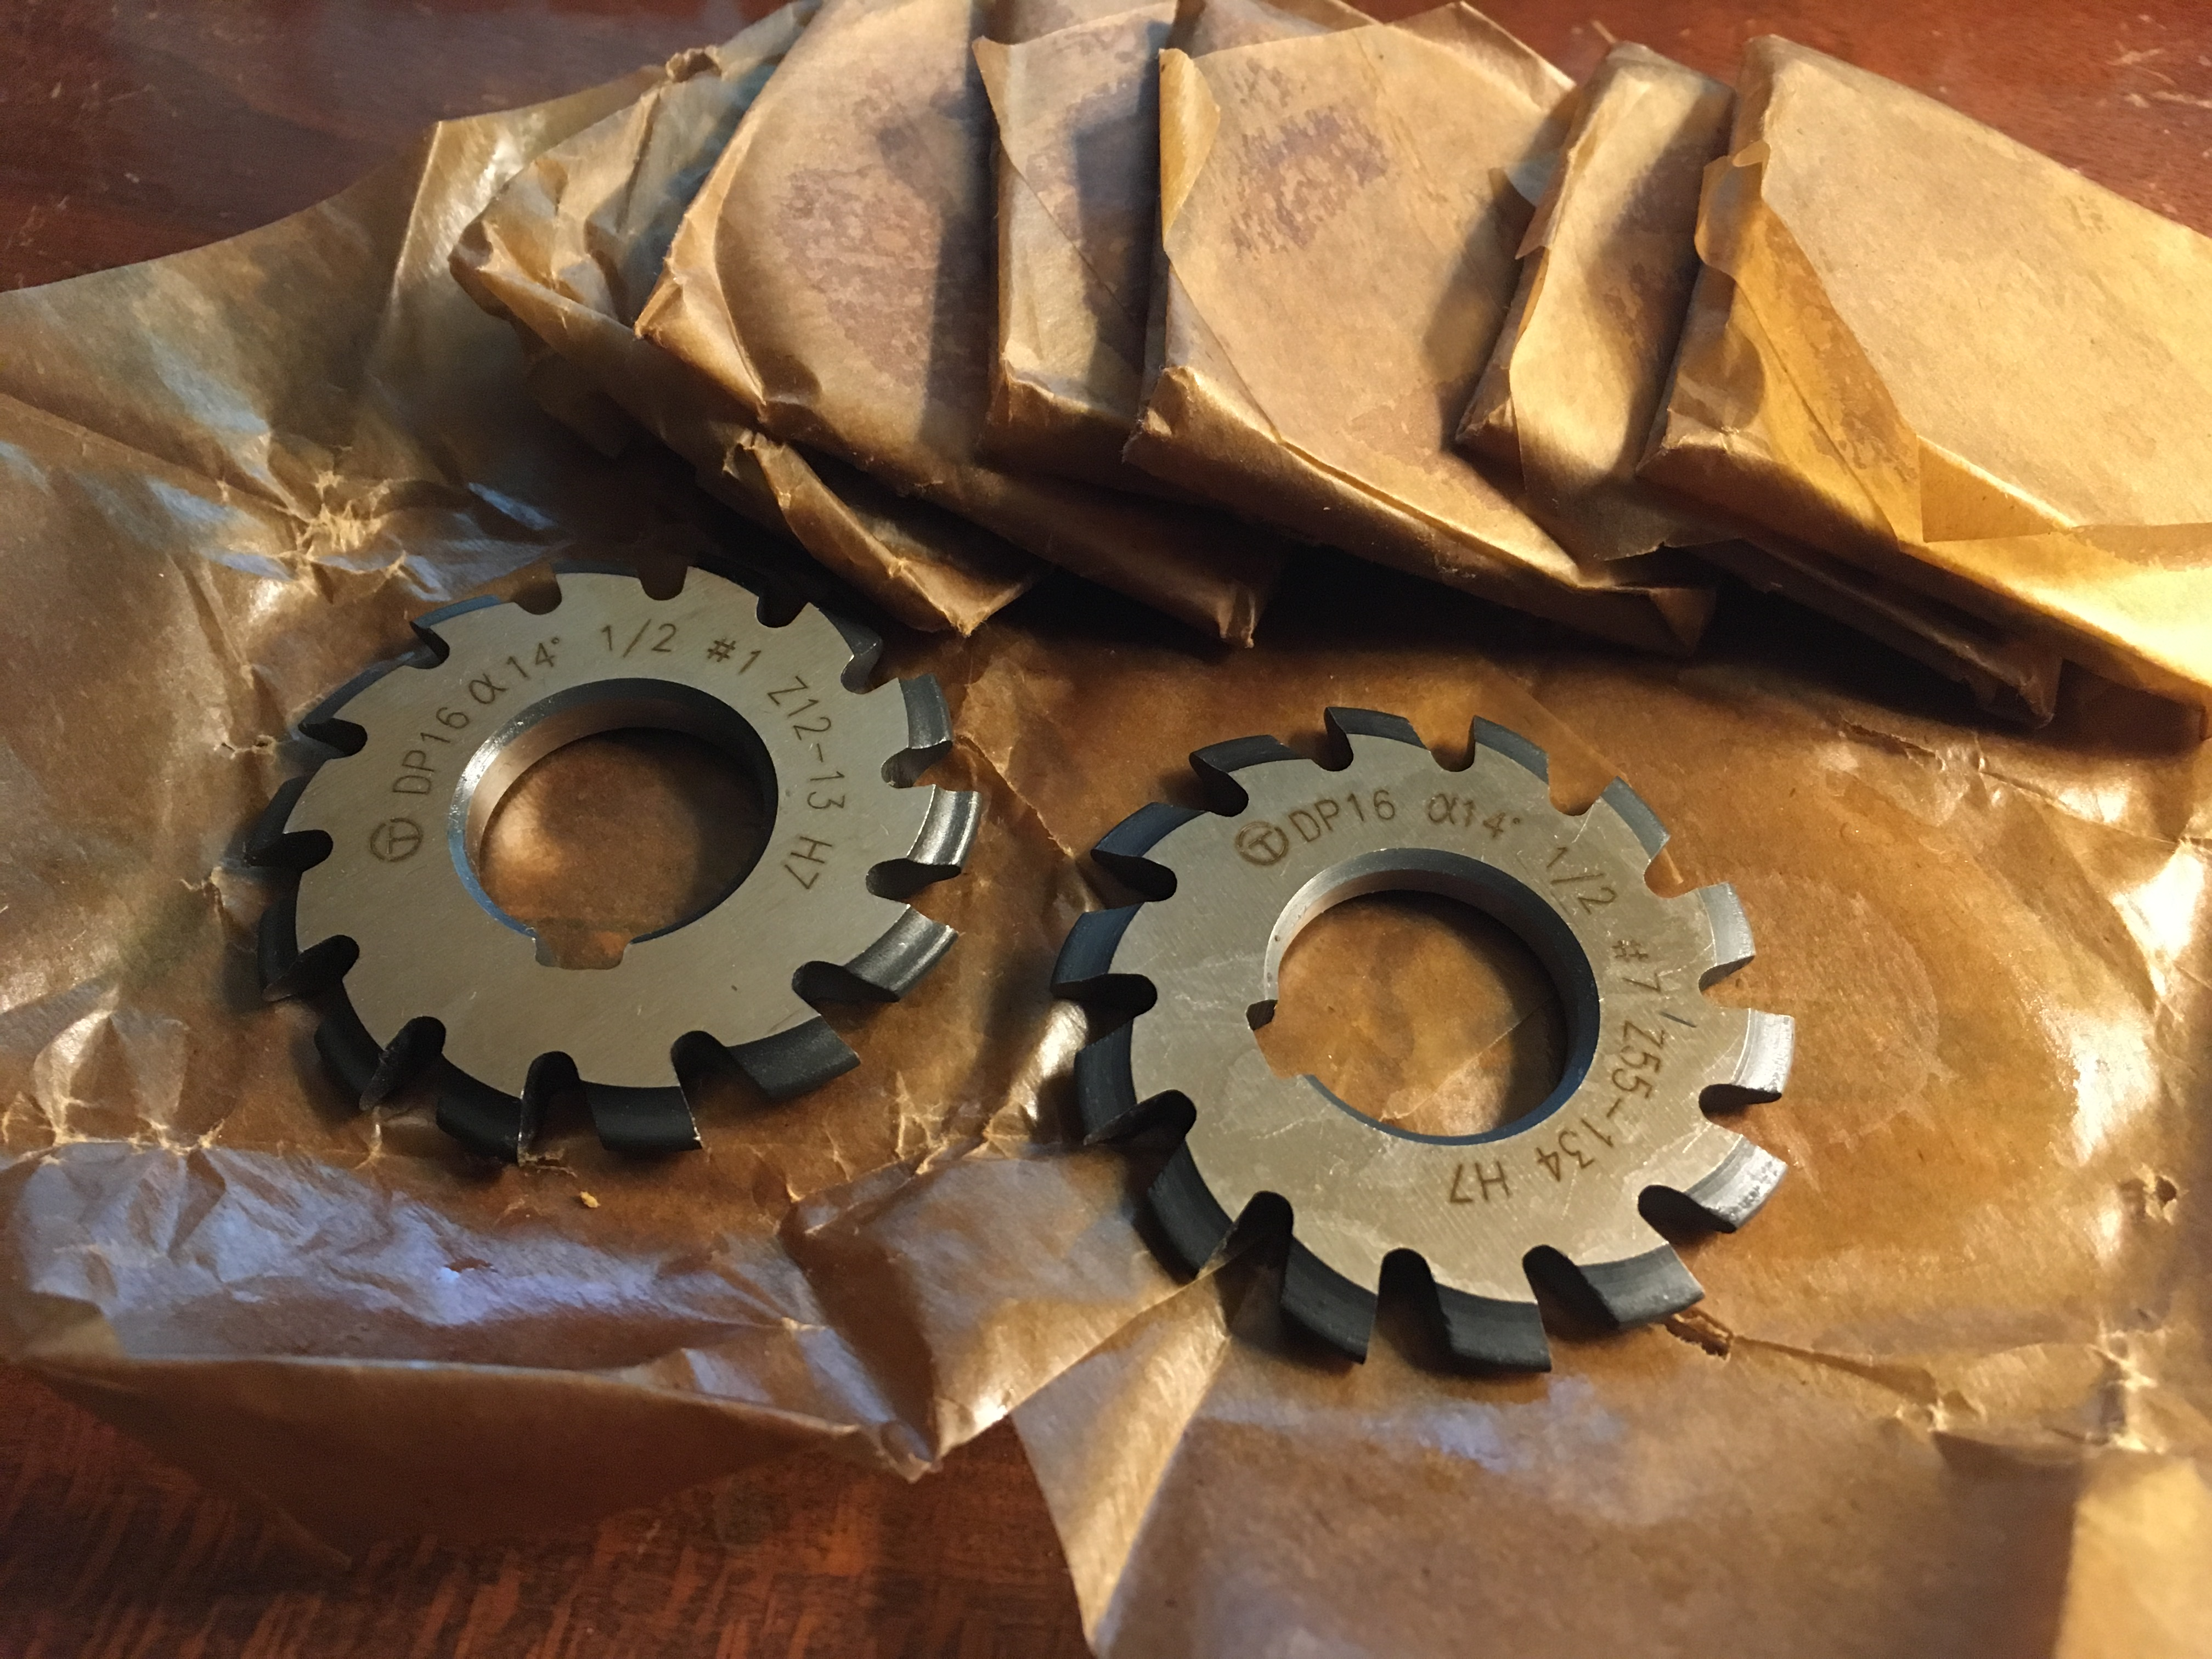
\includegraphics[width=5in]{cutter2}
	\caption{Series of Gear Cutters, for 16dp.}
\end{figure}

\subsubsection{Depth of Cut}
The depth of cut will be the sum of the addendum, dedendum, and minimum clearance. For a 16 pitch, 16-tooth gear, that will be:

 
\subsubsection{Gear Wires}
One of the simplest and best ways to measure gearing is to use gear wires and a micrometer. Gear wires are sized to sit right on the pitch circle of the gear, so as to measure indirectly the circle of contact. The size of a gear wire should be about 1.728 divided by the diametral pitch of the gear (Horton, 1954, p. 845) There are pre-made gear wires accordingt to a standard developed by the Van Keuren company. In our case we are cutting a 16dp gear, which will use a wire of 0.10800 diameter. (Horton, 1954, p. 854)  If ground and hardened pins are not available, you may make your own, though more approximate results are to be expected. 
\begin{figure}[H]
\centering

\includegraphics[width=5in]{imgpending}
	\caption{Measuring a Gear over home-made Wires.}
\end{figure}

\subsubsection{Speed and Feed}

Speeds and feeds are vital parameters in milling operations. "Speed" refers to the spindle speed in RPM, and "feed" refers to the feed rate of the work into the cutter, generally given in ipm or inches per minute. Speed is calculated backwards from cutter diameter, as the ultimate parameter being controlled is the surface speed of the cutting edge, which is faster for a larger cutter at a given number of RPMs.

In our case, we have a cutter of 2.2 inches outer diameter, and according to machinery's handbook, we should be looking for between 50 to 100sfm (Horton, 1954, p. 1503), or surface feet per minute. To determine the speed in sfm, `S', of the outside of a cutter with diameter `D' at a level of rpm 'R', we can employ this formula:


	\[S \;sfm = \frac{\pi \times D \; in \times R \;rpm}{12 \; in/ft}\]

If we need to find the rotational speed instead, we rearrange the equation:

	\[R\; rpm= \frac{12 \times S \;sfm}{\pi \times D \;in}\]

So for a 2.2 inch cutter at the lower 50 spm speed, we have:

	\[86.81 \; rpm = \frac{12\;  in/ft \times 50\;  sfm }{\pi \times 2.2\;  in} \]

Doing the same thing with 100 rpm, we get 173.62 rpm, so the spindle speed should be somewhere between 86.81 and 173.62 rpm. 
	 


\section{Machine Setup}
Machine setup is key to the gear cutting process going well. 



\subsection{Setting up the Index}
\begin{figure}[H]
\centering

\includegraphics[width=5in]{imgpending}
	\caption{Index and tailstock placed on the mill table.}
\end{figure}

\begin{itemize}
	\item Choose a dividing plate with the number of holes that you need to cut listed on it, or one that has the number of holes you need as a factor.
	\item Place the 10 inch horizontal index and the tailstock on the mill table.
	\item Align the index and tailstock roughly horizontally, and clamp lightly to the table.
	\item Set the cutting mandrel between centers for machine alignment.
	\item Use a dial indicator to ensure the height of the two centers is aligned - when run across the top of the mandrel, the dial indicator should show less than a thousandth runout.
	\item Use the dial indicator to verify horizontal alignment of the centers. When traversed across the mandrel, it should show less than a thousandth runout.
	\item When alignment is correct, clamp the tailstock firmly to the table.
\end{itemize}

\subsection{Setting up the Gear Blank}
\begin{figure}[H]
\centering

\includegraphics[width=5in]{imgpending}
\caption{Drawing showing gear blank set up in mill}
\end{figure}
\begin{itemize}
	\item Remove mandrel from index using screw on tailstock.
	\item Place gear blank on arbor. Tighten using a crescent wrench.
	\item Place lathe dog and copper shim on arbor. Be sure to use the copper shim to prevent marring the outside of the arbor.
	\item Tighten lathe dog in place using wrench.
	\item Place mandrel back between centers and mount snugly, using tailstock screw to cinch up on arbor.
	\item Tighten screw on dog driver plate to ensure setup does not come loose.
\end{itemize}


\subsection{Setting up the Cutter Arbor}
\begin{figure}[H]
\centering

\includegraphics[width=5in]{imgpending}
	\caption{Cutting Arbor Setup, with indications of major parts}
\end{figure}

\begin{itemize}
	\item Take the cutting arbor and place spacers on it until about half the space is taken up.
	\item Place the key in the arbor
	\item Place the cutter on the arbor, ensuring that it mates up with the key.
	\item Put the rest of the spacers on the arbor.
	\item Cinch up the cutter using the nut on the end of the arbor.
	\item Place the cutter arbor in the machine.
	\item Use the drawbar to hold the rear of the arbor firmly in the machine taper.
	\item Loosen the arm binders.
	\item Move the arbor support and the support arm so that the end of the arbor rests in the bearing hole of the support.
\end{itemize}

\subsection{Speeds and Feeds}
\begin{figure}[H]
\centering

\includegraphics[width=5in]{imgpending}
\caption{Photograph of speed and feed settings on machine.}
\end{figure}

\begin{itemize}
	\item Use the speed chart on the head of the mill to select the range corresponding to what was determined in section 1. In the example case, the ideal speed is 
	\item Place the key in the arbor
	\item Place the cutter on the arbor, ensuring that it mates up with the key.
	\item Put the rest of the spacers on the arbor.
	\item Cinch up the cutter using the nut on the end of the arbor.
	\item Place the cutter arbor in the machine.
	\item Use the drawbar to hold the rear of the arbor firmly in the machine taper.
	\item Loosen the arm binders.
	\item Move the arbor support and the support arm so that the end of the arbor rests in the bearing hole of the support.
\end{itemize}



\subsection{Table Stops}
\begin{figure}[H]
\centering

\includegraphics[width=5in]{imgpending}
	\caption{Photograph of table stops.}
\end{figure}

\begin{itemize}
\item Ensure that the cutter is above the workpiece. If not, lower the table until the cutter is above the workpiece.
\item Crank the main table feed over until the cutter is past the exit point of the gear. This is when the lowest point of the cutter has passed the left hand side of the gear.
\item Take a table stop and fasten it in the t-slot above the trip point (SP?)
\item Crank the main table feed over until the cutter is before the entry point of the gear. This is where no part of the cutter will be touching the gear.
\item Fasten a table stop in the t-slot at the beginning of the cut.
\item Ensure that the cutter is above the workpiece.
\item Start the table feed motor.
\item Engage automatic feed using lever, and ensure that it trips at the end of the cut.
\item Engage automatic feed in reverse using lever, and ensure that it trips at the beginning of the cut.
\item The automatic feed is now set up.
\end{itemize}
	

\subsection{Centering and Zeroing the Cutter}
	There are a number of methods for centering the milling cutter, but we will choose one requiring a minimum of measuring tools. It is ideal to do this with an indicator or a DRO, and it is generally frowned upon to use the dials for direct measurement. Nevertheless, here is a procedure for doing just that, in case another means of centering is not available:

\begin{enumerate}
\item Using the square on the mill table, align the rear edge of the cutter with the corresponding rear point on the edge of the gear blank (see figure below.) 
\item Find the offset W using cutter thickness T and gear blank diameter D: \[ W = \frac{1}{2} T \times D\]
\item Crank the table cross feed back by the dimension calculated.
\item Engage the saddle binder.
\item Loosen the cross feed collar and set the dial to zero. 
\item Center the part longitudinally, by eye only, using the table handwheel.
\item Start the spindle.
\item Raise the table to the cutter using the vertical feed handwheel until the cutter just touches off the top of the blank. It should barely scratch the surface. This is the vertical zero point.
\item Stop the machine using the 'stop' button.
\item Engage the knee binder.
\item Loosen the vertical feed collar and set the dial to zero. 

\end{enumerate}

\begin{figure}[H]
\centering

\includegraphics[width=5in]{imgpending}
	\caption{Aligning the cutter and the gear blank using a machinist's square.}
\end{figure}



\section{Gear Cutting}
\subsection{First Cut and finding the Zero Point}
\begin{enumerate}
\item Lower the vertical feed by .100
\item Place the work to the left of the cutter using the table feed handwheel.
\item Raise the work by .100, until dial reaches zero.
\item Raise the work by the intended depth of cut.
\item Engage knee binder.
\item Apply lubricant or engage cutting fluid pump.
\item Start spindle and automatic feed motor.
\item Engage table power feed lever.
\item Wait for the automatic table feed to trip, machine should make cut automatically.
\item Stop spindle, table motor, and coolant.
\item Lower the vertical feed by .100
\item Use table hand wheel to feed work out from under spindle.
\item Pause. Think. Is the spindle stopped? If it isn't, stop it now. This is an important place where you could get hurt if you don't stop the machine.
\item While in machine, measure cut using one gear wire and the back end of the gear blank. 
\item Determine how far off the measurement is from the ideal measurement. Adjust the vertical feed by the amount that the measurement is off.
\item Return to beginning of cut position using the table feed handwheel.
\item Raise the vertical feed to the cutting position, plus any offset calculated from the measurement.
\item Engage spindle and coolant (or brush on some more cutting fluid.)
\end{enumerate}

\subsection{Cutting the Rest of the Teeth}
The rest of the cuts are where the routine work sets in. Each gap in the gear is cut individually, and the gear rotated using the index between cuts. 
\begin{enumerate}
\item Ensure that the sector arms of the index and the pin are in the correct places as per the setup section.
\item Place the rear of the sector arm just counterclockwise of the index pin.
\item Pull the index pin out and move it clockwise until it rests in the hole just counterclockwise of the second index arm.
\item Move the rear index arm to touch the index pin again.
\item Apply cutting fluid if not working with a coolant system.
\item Engage automatic table feed, wait for cut to complete.
\item Disengage knee binder.
\item Drop table by .100
\item Feed table in reverse, either by hand or automatic feed.
\item Raise table by .100
\item Engage knee binder.
\item Are all teeth cut? If not, Return to step 1. Else, continue on to verifying the measurements of the gear.
\end{enumerate}

\section{Verifying Measurements}

\begin{enumerate}
\item Stop the mill spindle.
\item Using table feed, move gear blank out from under the spindle.
\item With gear still on mandrel, measure gear across wires using the micrometer.
\item With any luck, the gear should be the correct size. If it is too large, you can go back and take off a few thousandths by repeating the same procedure with the table raised by half the error (that is, if it is .004 too big, raise the table .002, because we cut on the radius. Don't cut off twice the error!) 
\item Once the gear is the appropriate size, remove it from the mill by unlocking the tailstock and unscrewing the center handle.
\item Dismount the gear from the mandrel by unscrewing the mounting nut.

\end{enumerate}

\section{Deburring and Cleanup}
\begin{enumerate}
\item Place the gear in a vise and use fine files to deburr and chamfer the edges of the cut.
\item Be sure to clean up all chips and wipe down the machine after use. This ensures everything is ready for setting up the next job!
\end{enumerate}


\section{Bibliography}

\begin{itemize}
	\item Installation, Operation, and Maintenance Instructions and Parts List for No. 16 Van Norman Ram Type Milling Machine Plain and Universal Models'' [Pamphlet]. (1952). Springfield, MA: Van Norman Company. 

	\item Horton, H. L. (Ed.). (1954). Machinery's Handbook (15th ed.). New York, NY: The Industrial Press. 

\end{itemize}

\end{document}
